\chapter{Numerical Linear Algebra tools}

\section{Introduction: Recap of Linear Algebra}

In this section we will review some basic concepts of Linear Algebra that will be useful for the rest of the course.

\subsection{Matrix-vector multiplication}

Given a matrix $A \in \mathbb{R}^{m \times n}$ and a vector $x \in \mathbb{R}^n$, the matrix-vector multiplication $y = Ax$ 
is defined as:

\begin{equation}
    y_i = \sum_{j=1}^{n} A_{ij} x_j
\end{equation}

A matrix-vector multiplication can be considered as a linear combination of the columns of the matrix $A$. Lets
see an example:

\begin{equation}
    \begin{bmatrix}
        1 & 4 \\
        2 & 5 \\
        3 & 6
    \end{bmatrix} \begin{bmatrix}
        x_1 \\
        x_2 \\
    \end{bmatrix} = \begin{bmatrix}
        1 \\
        2 \\
        3
    \end{bmatrix} x_1 + \begin{bmatrix}
        4 \\
        5 \\
        6
    \end{bmatrix} x_2
\end{equation}

\subsection{Column space of a matrix}

The column space of a matrix $A \in \mathbb{R}^{m \times n}$ is the subspace of $\mathbb{R}^m$ spanned by the columns of $A$.
In other words, it is the set of all possible linear combinations of the columns of $A$. The column space of a matrix is denoted
as $C(A)$.\\

If the columns of $A$ are linearly independent, then the column space of $A$ is the entire $\mathbb{R}^m$. If the columns of $A$
are linearly dependent, then the column space of $A$ is a subspace of $\mathbb{R}^m$ with dimension equal to the rank of $A$.\\

The rank of a matrix $A$ is is the size of the largest set of linearly independent columns of $A$. It is denoted as $rank(A)$.
Note that $rank(A) = rank(A^T)$.

\subsection{System of linear equations}

A system of linear equations is a set of $m$ equations with $n$ unknowns of the form:

\begin{equation}
    \begin{aligned}
        a_{11} x_1 + a_{12} x_2 + \ldots + a_{1n} x_n &= b_1 \\
        a_{21} x_1 + a_{22} x_2 + \ldots + a_{2n} x_n &= b_2 \\
        \vdots \\
        a_{m1} x_1 + a_{m2} x_2 + \ldots + a_{mn} x_n &= b_m \\
    \end{aligned}
\end{equation}

This system can be written in matrix form as $Ax = b$, where $A \in \mathbb{R}^{m \times n}$, $x \in \mathbb{R}^n$ 
and $b \in \mathbb{R}^m$.\\

The system $Ax = b$ has a solution if and only if $b \in C(A)$. If $b \in C(A)$, then the system has a unique solution
if and only if $rank(A) = n$. If $rank(A) < n$, then the system has infinitely many solutions.

\subsection{CR factorization}

The CR factorization of a matrix $A \in \mathbb{R}^{m \times n}$, with $m \geq n$, is a factorization of $A$ as $A = CR$, where
$C \in \mathbb{R}^{m \times r}$ is a matrix with the linearly independent columns of $A$ and $R \in \mathbb{R}^{r \times n}$ is 
obtained by determining the coefficients of the linear combination of the columns of $C$ that give the columns of $A$.
In this factorization, $r = rank(A)$.\\

Lets see an example:

\begin{equation}
    A = \begin{bmatrix}
        1 & 4 & 7 \\
        2 & 5 & 8 \\
        3 & 6 & 9
    \end{bmatrix} = \begin{bmatrix}
        1 & 4 \\
        2 & 5 \\
        3 & 6
    \end{bmatrix} \begin{bmatrix}
        1 & 0 & -1 \\
        0 & 1 & 2
    \end{bmatrix} = C R
\end{equation}

The matrix $C$ is also called the Row Reduced Echelon Form of $A$.

\subsection{Matrix-matrix multiplication}

Given two matrices $A \in \mathbb{R}^{m \times n}$ and $B \in \mathbb{R}^{n \times p}$, the matrix-matrix multiplication $C = AB$
is defined as:

\begin{equation}
    C_{ij} = \sum_{k=1}^{n} A_{ik} B_{kj}
\end{equation}

A matrix-matrix multiplication can be considered as the outer product of the columns of $A$ and the rows of $B$. Lets see an example:

\begin{equation}
    \begin{bmatrix}
        1 & 4 \\
        2 & 5 \\
        3 & 6
    \end{bmatrix} \begin{bmatrix}
        1 & 2 \\
        3 & 4
    \end{bmatrix} = \begin{bmatrix}
        1 \\
        2 \\
        3
    \end{bmatrix} \begin{bmatrix}
        1 & 2
    \end{bmatrix} + \begin{bmatrix}
        4 \\
        5 \\
        6
    \end{bmatrix} \begin{bmatrix}
        3 & 4
    \end{bmatrix}
\end{equation}

Note that each outer product generates a matrix of the same size as the result matrix, but always with rank 1. So 
the matrix-matrix multiplication can be considered as a sum of rank 1 matrices, obtained by the outer products of the columns of $A$
and the rows of $B$.

\subsection{Null space of a matrix}

The null space of a matrix $A \in \mathbb{R}^{m \times n}$ is the set of all vectors $x \in \mathbb{R}^n$ such that $Ax = 0$.
The null space of a matrix is denoted as $N(A)$. It is also called the kernel of $A$, denoted as $ker(A)$.\\

Formally, we have that:

\begin{equation}
    N(A) = \{ x \in \mathbb{R}^n : Ax = 0 \}
\end{equation}

The null space of a matrix is a subspace of $\mathbb{R}^n$. The dimension of the null space of a matrix is called the nullity 
of the matrix.

\subsection{Fundamental subspaces of a matrix}

Given a matrix $A \in \mathbb{R}^{m \times n}$, we can define four fundamental subspaces:

\begin{itemize}
    \item The column space of $A$, denoted as $C(A)$
    \item The row space of $A$, denoted as $C(A^T)$
    \item The null space of $A$, denoted as $N(A)$
    \item The left null space of $A$, denoted as $N(A^T)$
\end{itemize}

These subspaces are related by the following properties:

\begin{equation}
    \begin{aligned}
        C(A) &\perp N(A^T) \\
        C(A^T) &\perp N(A) \\
    \end{aligned}
\end{equation}

They also satisfy the following dimensions properties:

\begin{equation}
    \begin{aligned}
        dim(C(A)) + dim(N(A)) &= n \\
        dim(C(A^T)) + dim(N(A^T)) &= m \\
    \end{aligned}
\end{equation}

This is known as the Rank-Nullity Theorem.

\subsection{Orthogonal matrices}

An orthogonal matrix is a square matrix $Q \in \mathbb{R}^{n \times n}$ such that $Q^T Q = I$, where $I$ is the identity matrix.
This implies that $Q^T = Q^{-1}$.\\

Now, consider that $Q$ is an orthogonal matrix, and set $w = Q^T x$. Then we have that:

\begin{equation}
    \begin{aligned}
        \|w\|^2 =w^T w &= x^T Q Q^T x \\
        &= x^T x = \|x\|^2
    \end{aligned}
\end{equation}

This means that the norm of a vector is preserved under an orthogonal transformation. This is called an isometry. It is
a useful property for numerical algorithms, as it helps to avoid numerical instability.\\

There are two main types of orthogonal transformations that we are interested:

\subsubsection{Rotation matrices}

A rotation matrix is an orthogonal matrix that represents a rotation in $\mathbb{R}^2$ or $\mathbb{R}^3$. In $\mathbb{R}^2$,
a rotation matrix is of the form:

\begin{equation}
    Q(\theta) = \begin{bmatrix}
        \cos(\theta) & -\sin(\theta) \\
        \sin(\theta) & \cos(\theta)
    \end{bmatrix}
\end{equation}

\subsubsection{Reflection matrices}

A reflection matrix is an orthogonal matrix that represents a reflection with respect to a hyperplane. If $n$ denotes
the unit normal vector to the hyperplane, then the reflection matrix is of the form:

\begin{equation}
    Q = I - 2 n n^T
\end{equation}

Note that the inverse of this matrix is itself, as $Q^T = Q^{-1}$ and in this case, $Q$ is symmetric ($Q = Q^T$).\\

\subsection{QR factorization}

The QR factorization of a matrix $A \in \mathbb{R}^{m \times n}$, with $m \geq n$, is a factorization of $A$ as $A = QR$, where
$Q \in \mathbb{R}^{m \times n}$ is an orthogonal matrix and $R \in \mathbb{R}^{n \times n}$ is an upper triangular matrix.\\

\subsubsection{Gram-Schmidt process}

The Gram-Schmidt process is a method to compute the QR factorization of a matrix. Given a matrix $A \in \mathbb{R}^{m \times n}$,
the Gram-Schmidt process computes an orthonormal basis for the column space of $A$, as follows:

\begin{equation}
    \begin{aligned}
        q_1 &= \frac{a_1}{\|a_1\|} \\
        q_i = a_i - \sum_{j=1}^{i-1} &(q_j^T a_i) q_j \quad \forall i = 2, \ldots, n
    \end{aligned}
\end{equation}

where $a_i$ denotes the $i$-th column of $A$. The matrix $Q$ is obtained by stacking the vectors $q_i$ as columns. The matrix $R$
is obtained by computing the coefficients of the linear combination of the columns of $Q$ that give the columns of $A$.\\

\subsection{Eigenvalues and eigenvectors}

Given a square matrix $A \in \mathbb{R}^{n \times n}$, a scalar $\lambda$ is called an eigenvalue of $A$ if there exists a vector
$v \in \mathbb{R}^n$ such that:

\begin{equation}
    Av = \lambda v
\end{equation}

The vector $v$ is called an eigenvector of $A$ associated with the eigenvalue $\lambda$.\\

Let $P$ be the matrix whose columns are the eigenvectors of $A$, and $\Lambda$ be the diagonal matrix whose diagonal elements
are the eigenvalues of $A$. Then we have that:

\begin{equation}
    A = P \Lambda P^{-1}
\end{equation}

This is called the eigendecomposition of $A$.\\

The eigenvalues of a matrix are the roots of the characteristic polynomial of $A$, which is defined as:

\begin{equation}
    det(A - \lambda I) = 0
\end{equation}

\subsection{Similar matrices}

Two square matrices $A$ and $B$ are called similar if there exists a non-singular matrix $M$ such that:

\begin{equation}
    B = M^{-1} A M
\end{equation}

Similar matrices have the same eigenvalues, but not necessarily the same eigenvectors. Let $(\lambda, y)$ be 
an eigenpair of $B$, then we have:

\begin{equation}
    B y = \lambda y \Rightarrow M^{-1} A M y = \lambda y \Rightarrow A (M y) = \lambda (M y)
\end{equation}

This means that $M y$ is an eigenvector of $A$ associated with the eigenvalue $\lambda$. So, to obtain
the eigenvectors of $A$ from the eigenvectors of $B$, we need to multiply the eigenvectors of $B$ by $M$.\\

This property can be useful. For example, if we want to compute the eigenvalues of a matrix $A$, we can find
some transformation $M$ such that $M^{-1} A M = B$ is a simpler matrix to work with, usually a lower triangular
matrix. Then we can compute the eigenvalues of $B$ and obtain the eigenvalues of $A$. $M$ is obtained by the permutation
matrices to get from $A$ to $B$. The Givens and Householder transformations are examples of such method.

\section{Power method}

The power method is an iterative algorithm to compute the dominant eigenvalue of a matrix (i.e., the eigenvalue with the largest
magnitude). The algorithm is as follows:

\begin{algorithm}[H]
    \caption{Power method}
    \begin{algorithmic}[1]
        \State Choose a random vector $x^{(0)}$, s.t. $\|x^{(0)}\| = 1$
        \For{$k = 1, 2, \ldots$}
            \State $y^{(k)} = A x^{(k-1)}$
            \State $x^{(k)} = \frac{y^{(k)}}{\|y^{(k)}\|}$
            \State $\lambda^{(k)} = x^{(k)T} A x^{(k)}$
        \EndFor
    \end{algorithmic}
\end{algorithm}

The convergence rate is determined by the ratio of the largest eigenvalue to the 
second largest eigenvalue.

\subsection{Rayleigh quotient}

The Rayleigh quotient is the base of the power method algorithm. Given a matrix $A \in \mathbb{R}^{n \times n}$ and
a vector $x \in \mathbb{R}^n$, the Rayleigh quotient is defined as:

\begin{equation}
    R(x) = \frac{x^T A x}{x^T x}
\end{equation}

For every eigenpair $(\lambda, v)$ of $A$, we have that:

\begin{equation}
    R(v) = \frac{v^T A v}{v^T v} = \frac{v^T \lambda v}{v^T v} = \lambda
\end{equation}

This means that the Rayleigh quotient is equal to the eigenvalue associated with the eigenvector $v$. This property
is used in the power method to compute the dominant eigenvalue of a matrix.

\subsection{Proof of convergence for the power method}

The power method converges to the dominant eigenvalue of a matrix. The sketch proof is as follows:\\

Let $x^{(0)}$ be our initial vector, and let $\{v_1, \ldots, v_n\}$ be the eigenvectors of $A$. We can write $x^{(0)}$ as a linear
combination of the eigenvectors of $A$ (since the eigenvectors of $A$ form a basis of $\mathbb{R}^n$):

\begin{equation}
    x^{(0)} = \sum_{i=1}^{n} \alpha_i v_i
\end{equation}

Then we have that:

\begin{equation}
    A x^{(0)} = \sum_{i=1}^{n} \alpha_i A v_i = \sum_{i=1}^{n} \alpha_i \lambda_i v_i
\end{equation}

Since in every iteration $k$ of the power method we apply the matrix $A$ to the vector $x^{(k-1)}$, we have that:

\begin{equation}
    A x^{(k-1)} = A^k x^{(0)} = \sum_{i=1}^{n} \alpha_i \lambda_i^k v_i
\end{equation}

Now, let us factorize the previous equation by the dominant eigenvalue $(\lambda_1)^k$:

\begin{equation}
    A^k x^{(0)} = (\lambda_1)^k \left( \alpha_1 v_1 + \sum_{i=2}^{n} \alpha_i \left( \frac{\lambda_i}{\lambda_1} \right)^k v_i\right)
\end{equation}

Note that the term inside the parenthesis converges to zero as $k \rightarrow \infty$, since the ratio of the other eigenvalues
to the dominant eigenvalue is less than 1. This means that $x^(k)$ converges to the direction of the dominant eigenvector $v_1$.
When it is normalized, its Rayleigh quotient converges to the dominant eigenvalue $\lambda_1$.

\subsection{Inverse power method}

The inverse power method is an iterative algorithm to compute the eigenvalue with the smalles magnitude of a matrix. Note that the smallest
eigenvalue of a matrix is the largest eigenvalue of its inverse, since:

\begin{equation}
    A x = \lambda x \Rightarrow A^{-1} x = \frac{1}{\lambda} x
\end{equation}

The algorithm is similar to the power method, but instead of applying the matrix $A$ to the vector $x$, we apply the inverse
of the matrix $A$:

\begin{algorithm}[H]
    \caption{Inverse power method}
    \begin{algorithmic}[1]
        \State Choose a random vector $x^{(0)}$, s.t. $\|x^{(0)}\| = 1$
        \For{$k = 1, 2, \ldots$}
            \State $y^{(k)} = A^{-1} x^{(k-1)}$
            \State $x^{(k)} = \frac{y^{(k)}}{\|y^{(k)}\|}$
            \State $\lambda^{(k)} = x^{(k)T} A x^{(k)}$
        \EndFor
    \end{algorithmic}
\end{algorithm}

In practice, we normally don't compute the inverse of the matrix $A$, but instead solve the linear system $A x = y^{(k)}$ in each
iteration.

\subsection{Shifted inverse power method}

The shifted inverse power method is an iterative algorithm to compute the eigenvalue with the smalles magnitude of a matrix, but
with a shift $\mu$ added to the matrix $A$. The algorithm is as follows:

\begin{algorithm}[H]
    \caption{Shifted inverse power method}
    \begin{algorithmic}[1]
        \State Choose a random vector $x^{(0)}$, s.t. $\|x^{(0)}\| = 1$
        \For{$k = 1, 2, \ldots$}
            \State $y^{(k)} = (A - \mu I)^{-1} x^{(k-1)}$
            \State $x^{(k)} = \frac{y^{(k)}}{\|y^{(k)}\|}$
            \State $\lambda^{(k)} = x^{(k)T} A x^{(k)}$
        \EndFor
    \end{algorithmic}
\end{algorithm}

Note that with this algorithm, we are computing the eigenvalue of $A$ that is closest to the shift $\mu$. This can be useful
to compute the eigenvalues of a matrix that are close to a given value.

\section{Symmetric matrices}

A matrix $A \in \mathbb{R}^{n \times n}$ is called symmetric if $A = A^T$. Symmetric matrices have important properties:

\begin{itemize}
    \item The eigenvectors of a symmetric matrix form an orthonormal basis of $\mathbb{R}^n$.
    \item All the eigenvalues of a symmetric matrix are real.
\end{itemize}

Let us prove the first property:\\

Let $A$ be a symmetric matrix, and let $\lambda_1, \ldots, \lambda_n$ be its eigenvalues. Let $v_1, \ldots, v_n$ be the eigenvectors
associated with the eigenvalues $\lambda_1, \ldots, \lambda_n$. Let us take two eigenvectors $v_i$ and $v_j$, such that $i \neq j$.
Then we have that:

\begin{equation}
    A v_i = \lambda_i v_i \quad \text{and} \quad A v_j = \lambda_j v_j
\end{equation}

Then we have that:

\begin{equation*}
    (A - \lambda_i I) v_i = 0 \quad \text{and} \quad (A - \lambda_i I) v_j = (\lambda_j - \lambda_i) v_j 
\end{equation*}

\begin{equation}
    \Rightarrow v_i \in N(A - \lambda_i I) \quad \text{and} \quad v_j \in C(A - \lambda_i I)
\end{equation}

Since $A$ is symmetric, we have that $A - \lambda_i I$ is also symmetric. Then we have that:

\begin{equation}
    N(A - \lambda_i I) = N((A - \lambda_i)^T) \perp C(A - \lambda_i I)
\end{equation}

Concluding that $v_i$ and $v_j$ are orthogonal. Since this holds for all pairs of eigenvectors, we have that the eigenvectors
of a symmetric matrix form an orthonormal basis of $\mathbb{R}^n$.\\

Now, let us prove the second property:\\

Since $A$ is symmetric, we have that $A = A^T$. Then we have that:

\begin{equation}
    \begin{aligned}
        A x &= \lambda x \\
        A \bar{x} &= \bar{\lambda} \bar{x}
    \end{aligned}
\end{equation}

Then we have that:

\begin{equation}
    \begin{aligned}
        \bar{x}^T A x &= \lambda x^T x = \lambda \|x\|^2 \\
        x^T A \bar{x} &= \bar{\lambda} x^T \bar{x} = \bar{\lambda} \|x\|^2
    \end{aligned}
\end{equation}

Since $A = A^T$, we have that:

\begin{equation}
    \bar{x}^T A x = (A x)^T \bar{x} = x^T A^T \bar{x} = x^T A \bar{x}
\end{equation}

Then we have that:

\begin{equation}
    \lambda \|x\|^2 = \bar{\lambda} \|x\|^2 \Rightarrow \lambda = \bar{\lambda}
\end{equation}

This means that the eigenvalues of a symmetric matrix are real.

\subsection{Symmetric positive definite matrices}

A matrix $A \in \mathbb{R}^{n \times n}$ is called symmetric positive definite if it is symmetric and if for every vector $x \in \mathbb{R}^n$
we have that:

\begin{equation}
    x^T A x > 0 \quad \forall x \neq 0
\end{equation}

Symmetric positive definite matrices have important properties:

\begin{itemize}
    \item All the eigenvalues of a symmetric positive definite matrix are positive.
    \item The Cholesky factorization of a symmetric positive definite matrix exists and is unique:
    \begin{equation}
        A = L^T L
    \end{equation}
\end{itemize}

In fact, a symmetric matrix is positive definite if and only if all its eigenvalues are positive, so:

\begin{equation}
    x^T A x > 0 \quad \forall x \neq 0 \quad \Leftrightarrow \quad \lambda_i > 0 \quad \forall i
\end{equation}

Note that the quantity $x^T A x$ is called the energy of the vector $x$ with respect to the matrix $A$. This quantity is always positive
for a symmetric positive definite matrix.\\


\section{Singular Value Decomposition (SVD)}

The Singular Value Decomposition (SVD) is a factorization of a matrix $A \in \mathbb{R}^{m \times n}$ as:

\begin{equation}
    A = U \Sigma V^T
\end{equation}

where $U \in \mathbb{R}^{m \times m}$ and $V \in \mathbb{R}^{n \times n}$ are orthogonal matrices, and $\Sigma \in \mathbb{R}^{m \times n}$
is a quasi-diagonal matrix with the singular values of $A$. The singular values of $A$ are the square roots of the eigenvalues of $A^T A$.\\

Note that if $rank(A) = r$, then the matrix $\Sigma$ has $r$ non-zero singular values, and the remaining singular values are zero. Assume that
the singular values of $A$ are $\sigma_1 \geq \sigma_2 \geq \ldots \geq \sigma_r > 0$. Then we have that:

\begin{equation}
    \begin{aligned}
        A v_i &= \sigma_i u_i \quad \forall i = 1, \ldots, r \\
        A v_i &= 0 \quad \forall i = r+1, \ldots, n \\
    \end{aligned}
\end{equation}

where $u_i$ and $v_i$ are the columns of $U$ and $V$, respectively. The vectors $u_i$ and $v_i$ are called the left and right singular vectors
of $A$, respectively.\\

The SVD can also be written as:

\begin{equation}
    A = \sum_{i=1}^{r} \sigma_i u_i v_i^T
\end{equation}

\subsection{Economy SVD}

The economy SVD is a factorization of a matrix $A \in \mathbb{R}^{m \times n}$ as:

\begin{equation}
    A = U_r \Sigma_r V_r^T
\end{equation}

where $U \in \mathbb{R}^{m \times r}$, $V \in \mathbb{R}^{n \times r}$ and $\Sigma \in \mathbb{R}^{r \times r}$, with $r = rank(A)$.\\

The economy SVD is useful when we are only interested in the first $r$ singular values of $A$, which are the non-zero singular values.\\

\subsection{Low-rank approximation}

The SVD can be used to compute a low-rank approximation of a matrix $A \in \mathbb{R}^{m \times n}$. Given a rank $k$, with $k < r = rank(A)$,
the low-rank approximation of $A$ is given by:

\begin{equation}
    A_k = U_k \Sigma_k V_k^T = \sum_{i=1}^{k} \sigma_i u_i v_i^T
\end{equation}

where $U_k \in \mathbb{R}^{m \times k}$, $V_k \in \mathbb{R}^{n \times k}$ and $\Sigma_k \in \mathbb{R}^{k \times k}$, with $k < r = rank(A)$.\\

Because the singular values of $A$ are sorted in decreasing order, the low-rank approximation only considers the first $k$ singular values of $A$,
as they are the components of $A$ with the largest contribution.\\

The low-rank approximation of a matrix is useful for data compression, as it allows to represent a matrix with a smaller number of parameters. 
Note that the low-rank approximation of a matrix is the best rank-$k$ approximation of the matrix in the Frobenius norm. This is called 
the Eckart-Young theorem.

\subsubsection{Optimal thresholding for low-rank approximation}

There are several methods to determine the optimal rank $k$ for the low-rank approximation of a matrix. A common heuristic approach
is to graph the singular values of the matrix and choose the rank $k$ as the point where the singular values start to decay rapidly.\\

We can see the idea of this method in the following figure:\\

\begin{figure}[H]
    \centering
    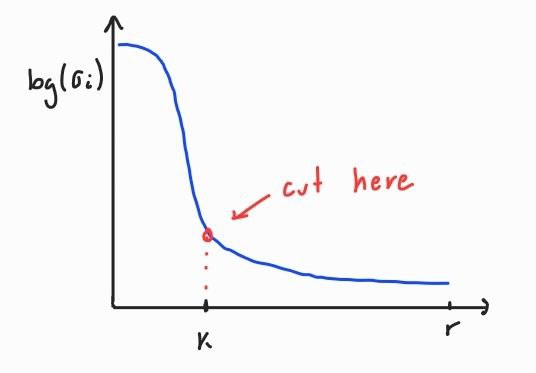
\includegraphics[width=0.4\textwidth]{figures/image_opt_thresh_1.jpg}
    \caption{Heuristic method for choosing $k$}
    \label{fig:heur_k_choose}
\end{figure}

Another common method is to use the cumulative energy of the singular values. The cumulative energy is defined as:

\begin{equation}
    \frac{\sum_{i=1}^{k} \sigma_i^2}{\sum_{i=1}^{r} \sigma_i^2}
\end{equation}

The cumulative energy measures the proportion of the total energy of the matrix that is captured by the first $k$ singular values. A common
heuristic is to choose the rank $k$ as the smallest value such that the cumulative energy is above a certain threshold, e.g., 90\%.\\

However, the optimal rank $k$ for the low-rank approximation of a matrix is a complex problem that depends on the specific application.
For example, we can use the following model:

\begin{equation}
    A = A_{TRUE} + \gamma A_{NOISE}
\end{equation}

where $A_{TRUE}$ is the true low-rank matrix that we want to approximate, $A_{NOISE}$ is the noise matrix, and $\gamma$ is the noise level.
In this case, the optimal rank $k$ is the one that minimizes the error of the low-rank approximation of $A_{TRUE}$.\\

For this case, depending of the knowledge of the noise level, we can use the following methods to compute a threshold.

\begin{enumerate}
    \item If the noise level is known, and $A \in \R^{n \times n}$ is a square matrix, then we can use the following threshold:
    
    \begin{equation}
        \tau = \frac{4}{\sqrt{3}} \sqrt{n} \gamma
    \end{equation}

    \item If $n << m$:
    
    \begin{equation}
        \tau = \lambda{\frac{n}{m}} \sqrt{n}
    \end{equation}

    Where $\lambda(\cdot)$ is a computable function (specific for this model, we don't care about it).

    \item $\gamma$ is unknown:
    
    \begin{equation}
        \tau = \omega(\frac{n}{m}) \sigma_{med}
    \end{equation}

    Where $\sigma_{med}$ is the median of the singular values of $A$, and $\omega(\cdot)$ is a computable function 
    (specific for this model, we don't care about it).
\end{enumerate}

The idea is to select the singular values that are above the threshold.

\subsection{Existance of the SVD}

The SVD of a matrix $A \in \mathbb{R}^{m \times n}$ always exists. The proof is as follows:\\

Let $A \in \mathbb{R}^{m \times n}$ be a matrix. Then we have that $A^T A \in \mathbb{R}^{n \times n}$.
We have that $A^T A$ is symmetric and positive semidefinite. In fact:

\begin{itemize}
    \item $A^T A$ is symmetric: $(A^T A)^T = A^T (A^T)^T = A^T A$
    \item $A^T A$ is positive semidefinite: $x^T A^T A x = (A x)^T A x = \|A x\|^2 \geq 0$
\end{itemize}

Therefore, $A^T A$ has an eigendecomposition:

$$A^T A = V \Lambda V^T \quad \text{s.t. } V^T V = I$$

Let us show now that $rank(A) = rank(A^T A)$. We can prove this by showing that the null space of $A$ 
is the same as the null space of $A^T A$. Let $x \in N(A)$, then we have that:

$$A x = 0 \Rightarrow A^T A x = 0$$

This means that $N(A) \subseteq N(A^T A)$. Now, let $x \in N(A^T A)$, then we have that:

$$A^T A x = 0 \Rightarrow x^T A^T A x = 0 \Rightarrow \|A x\|^2 = 0 \Rightarrow A x = 0$$

This means that $N(A^T A) \subseteq N(A)$. Therefore, $N(A) = N(A^T A)$, and we have 
that $rank(A) = rank(A^T A)$.\\

Now, let us consider the eigenpairs $(\lambda_i, v_i)$ of $A^T A$. Then let us define $u_i$ as:

$$u_i = \frac{1}{\sqrt{\lambda_i}} A v_i$$

We will prove that each $u_i$ is a unitary vector, and that the vectors $u_i$ are mutually orthogonal. 
Let us first show that each $u_i$ is a unitary vector:

$$\|u_i\|^2 = \left\| \frac{1}{\sqrt{\lambda_i}} A v_i \right\|^2 = \frac{1}{\lambda_i} v_i^T A^T A v_i = \frac{1}{\lambda_i} \lambda_i = 1$$

Now, let us show that the vectors $u_i$ are mutually orthogonal. Let $i \neq j$, then we have that:

$$u_i^T u_j = \frac{1}{\sqrt{\lambda_i}} v_i^T A^T \frac{1}{\sqrt{\lambda_j}} A v_j = \frac{1}{\sqrt{\lambda_i \lambda_j}} v_i^T A^T A v_j$$
$$= \frac{1}{\sqrt{\lambda_i \lambda_j}} \lambda_j v_i^T v_j = 0$$

Now, we can show that the vectors $u_i$ are the eigenvectors of $A A^T$, with eigenvalues
$\lambda_i$:

$$A A^T u_i = A A^T \frac{1}{\sqrt{\lambda_i}} A v_i = $$
$$\frac{1}{\sqrt{\lambda_i}} A A^T A v_i = \frac{1}{\sqrt{\lambda_i}} A \lambda_i v_i = \lambda_i u_i$$

Therefore, we have that $A A^T = U \Lambda U^T$, where $U$ is the matrix whose columns are the vectors $u_i$.
Now, let us define $\Sigma$ as the diagonal matrix whose diagonal elements are the square roots of the eigenvalues of $A^T A$:

$$\Sigma = \begin{bmatrix}
    \sqrt{\lambda_1} & 0 & \ldots & 0 \\
    0 & \sqrt{\lambda_2} & \ldots & 0 \\
    \vdots & \vdots & \ddots & \vdots \\
    0 & 0 & \ldots & \sqrt{\lambda_n}
\end{bmatrix}$$

Then we have that:

$$A = U \Sigma V^T$$

where $V$ is the matrix whose columns are the eigenvectors of $A^T A$. Therefore, the SVD of $A$ exists.

\subsection{Computation of the SVD}

The SVD of a matrix can be computed using the following steps:

\begin{enumerate}
    \item Compute the eigendecomposition of $A^T A$.
    \item Compute the singular values of $A$ as the square roots of the eigenvalues of $A^T A$.
    \item Compute the right singular vectors of $A$ as the eigenvectors of $A^T A$.
    \item Compute the left singular vectors of $A$ as $u_i = \frac{1}{\sqrt{\lambda_i}} A v_i$.
\end{enumerate}

\subsection{Geometrical interpretation of the SVD}

The SVD of a matrix $A \in \mathbb{R}^{m \times n}$ can be interpreted geometrically as a composition of three transformations:

\begin{itemize}
    \item The matrix $V$ represents a rotation in $\mathbb{R}^n$.
    \item The matrix $\Sigma$ represents a scaling in $\mathbb{R}^{m \times n}$.
    \item The matrix $U$ represents a rotation in $\mathbb{R}^m$.
\end{itemize}

In $\R^2$, the SVD of a matrix $A$ can be interpreted as a rotation of the unit circle, followed by a scaling along the axes, 
followed by another rotation. So this transformation can be represented with 4 parameters: two angles and two scaling factors.
In $\R^3$, its the same idea, but with 6 parameters: three angles and three scaling factors.

\subsection{Polar decomposition}

Let $A \in \R^{n \times n}$ be a symmetric matrix. The polar decomposition of $A$ is a factorization of $A$ as:

\begin{equation}
    A = Q S
\end{equation}

where $Q$ is an orthogonal matrix and $S$ is a symmetric positive definite matrix. 
The polar decomposition can be derived from the SVD of $A$ as:

\begin{equation}
    A = U \Sigma V^T = (U V^T) (V \Sigma V^T) = Q S
\end{equation}

where $Q = U V^T$ and $S = V \Sigma V^T$. So, the polar decomposition of a symmetric matrix
always exists.

\subsection{Eckart-Young theorem}

The Eckart-Young theorem states that the best rank-$k$ approximation of a matrix $A \in \mathbb{R}^{m \times n}$ in the Frobenius norm
is given by the low-rank approximation of $A$, denoted as $A_k$:

\begin{equation}
    \min_{rank(B) = k} \|A - B\|_F = \|A - A_k\|_F
\end{equation}

This also applies to the spectral norm $\| \cdot \|_2$. To prove this, let us define the mentioned
norms:

\subsubsection{Frobenius norm}

The Frobenius norm of a matrix $A \in \mathbb{R}^{m \times n}$ is defined as:

\begin{equation}
    \|A\|_F = \sqrt{\sum_{i=1}^{m} \sum_{j=1}^{n} A_{ij}^2}
\end{equation}

The Frobenius norm is the Euclidean norm of the vector obtained by stacking the columns of $A$.
It is also equal to:

\begin{equation}
    \|A\|_F = \sqrt{tr(A^T A)}
\end{equation}

It has 3 important properties:

\begin{enumerate}
    \item $\|A\|_F = \|A^T\|_F$
    \item It is invariant under orthogonal transformations: $\|Q A\|_F = \|A\|_F$
    \item It is equal to the square root of the sum of the squared singular values of $A$: 
    \begin{equation}
        \|A\|_F = \sqrt{\sum_{i=1}^{r} \sigma_i^2}
    \end{equation}
\end{enumerate}

\subsubsection{Spectral norm}

The spectral norm of a matrix $A \in \mathbb{R}^{n \times n}$ is defined as:

\begin{equation}
    \|A\|_2 = \sup_{\|x\|_2 = 1} \|A x\|_2
\end{equation}

It is equal to the largest singular value of $A$. This is denoted as:

\begin{equation}
    \|A\|_2 = \sigma_1
\end{equation}

\subsubsection{Proof of the Eckart-Young theorem}

For both norms $\| \cdot \|_F$ and $\| \cdot \|_2$, we will prove that:

$$\| A - A_k \| \leq \| A - B \| \quad \forall B \in \mathbb{R}^{m \times n} \quad \text{s.t.} \quad rank(B) = k$$

Let $B \in \mathbb{R}^{m \times n}$ be a matrix such that $rank(B) = k$. Then we have that:

$$dim(N(B)) = n - k$$

Let us consider the matrix $V_{k+1}$ whose columns are the vectors $v_{1}, \ldots, v_{k+1}$ 
from the SVD of $A$. Then we have that:

$$rank(V_{k+1}) = k+1 \Rightarrow dim(C(V_{k+1})) = k + 1$$
$$\Rightarrow dim(N(B)) + dim(C(V_{k+1})) = n - k + k + 1 = n + 1$$


This means that $N(B) \cap C(V_{k+1}) \neq \emptyset$. Let $w \in N(B) \cap C(V_{k+1})$, 
such that $\|w\| = 1$. Then we have that, for coefficients $\alpha_i$:

$$w = \sum_{i=1}^k \alpha_i v_i \quad \wedge \quad B w = 0$$

Since $\|w\| = 1$, then $\sum_{i=1}^k \alpha_i^2 = 1$. Now, we have that, for the 
spectral norm:

$$\|A - B\|_2^2 \geq \|(A - B) w\|_2^2 = \|A w\|_2^2 = w^T A^T A w$$
$$= w^T V \Sigma^2 V^T w = \sum_{i=1}^k \sigma_i^2 \alpha_i^2 \geq$$
$$\geq \sigma_{k+1}^2 \sum_{i=1}^k \alpha_i^2 = \sigma_{k+1}^2$$
$$= \|A - A_k\|_2^2$$

Therefore:

$$\|A - A_k\|_2 \leq \|A - B\|_2 \quad \forall B \in \mathbb{R}^{m \times n} \quad \text{s.t.} \quad rank(B) = k$$

For the Frobenius norm, we need to use the Weyl's inequality:

\begin{equation}
    \sigma_{i + j - 1}(X + Y) \leq \sigma_i(X) + \sigma_j(Y)
\end{equation}

where $\sigma_i(X)$ denotes the $i$-th singular value of a matrix $X$. Using this inequality, 
let us define $X = A - B$ and $Y = B$. Then we have that:

$$\sigma_{i + k}(A) \leq \sigma_i(A - B) + \sigma_{k + 1}(B)$$

Note that $\sigma_{k+1}(B) = 0$, since $B$ has rank $k$. Therefore:

$$\sigma_{i + k}(A) \leq \sigma_i(A - B)$$

Then, we have that:

$$\|A - A_k\|_F^2 = \sum_{i=k+1}^r \sigma_i^2(A) = \sum_{i=1}^{r - k} \sigma_{i+k}^2(A) \leq$$
$$\leq \sum_{i=1}^{r - k} \sigma_i^2(A - B) \leq \sum_{i=1}^n \sigma_i^2(A - B) = \|A - B\|_F^2$$

Therefore:

$$\|A - A_k\|_F \leq \|A - B\|_F \quad \forall B \in \mathbb{R}^{m \times n} \quad \text{s.t.} \quad rank(B) = k$$

This completes the proof.

\subsection{Principal Component Analysis (PCA)}

Principal Component Analysis (PCA) is a technique to reduce the dimensionality of a dataset. Given a dataset $X \in \mathbb{R}^{m \times n}$,
PCA computes the SVD of the centered data matrix $\bar{B}$, where $\bar{B}$ is obtained by subtracting the mean of each column of $X$.
Then, the principal components of the dataset are the right singular vectors of $\bar{B}$. The principal components are the directions
of the dataset with the largest variance.\\

In detail, let $X \in \R^{m \times n}$ the dataset, with $m$ samples and $n$ features. Let $\bar{x}$ be mean vector of the data samples.
Then, we define $\bar{X}$ as:

\begin{equation}
    \bar{X} = \begin{bmatrix}
        1 \\
        \vdots \\
        1
    \end{bmatrix} \bar{x}^T
\end{equation}

Then, we define the centered data matrix $\bar{B}$ as:

\begin{equation}
    \bar{B} = X - \bar{X}
\end{equation}

The covariance matrix is then defined as:

\begin{equation}
    C = \frac{1}{m - 1} \bar{B}^T \bar{B}
\end{equation}

We observe that the eigendecomposition of the covariance matrix $C$ is as follows:

\begin{equation}
    C = V \Lambda V^T
\end{equation}

We can obtain the principal components of the dataset as the columns of $V$. The principal components are the directions of the dataset
with the largest variance. The first principal component is the direction with the largest variance, the second principal component is
the direction with the second largest variance, and so on.\\

By doing the SVD of the centered data matrix $\bar{B}$, we can obtain the principal components of the dataset, such that:

\begin{equation}
    \bar{B} = U \Sigma V^T
    \Rightarrow V = \text{principal components} \quad \wedge \quad \Lambda = \frac{1}{m - 1} \Sigma^2 
\end{equation}

\subsection{Data pre-processing: sensitivity to transformations}

The SVD is specially sensitive to scaling, rotating and translating the data. This is because the SVD
is a geometrical transformation of the data, and these transformations change the geometry of the data.
For that reason, if we want to apply the SVD to a dataset, we need to pre-process the data to remove or somehow
filter the effects of these transformations.\\

For example, if we have a dataset that consist of face images, and we want to apply the SVD to this dataset,
we need to pre-process the images to remove the effects of scaling, rotating and translating the faces. This can
be done by aligning the faces to a common reference frame, and by normalizing the faces to have the same size and
orientation.\\

In general, the pre-processing of the data is an important step in the application of the SVD to a dataset. The
pre-processing step can have a significant impact on the results of the SVD, and it is important to carefully
choose the pre-processing steps to obtain meaningful results.

\subsection{Randomized SVD}

The SVD of a matrix can be computed using the randomized SVD algorithm. The randomized SVD is an iterative algorithm
that approximates the SVD of a matrix using random projections. The algorithm is as follows:

\begin{algorithm}[H]
    \caption{Randomized SVD}
    \begin{algorithmic}[1]
        \State Choose a random matrix $Y \in \mathbb{R}^{n \times k}$, with $k \ll n$.
        \State Compute the matrix $Z = A Y$.
        \State Compute the QR factorization of $Z = Q R$.
        \State Compute the matrix $B = Q^T A$.
        \State Compute the SVD of $B = \hat{U} \Sigma V^T$.
        \State Obtain $U$ as $U = Q \hat{U}$.
        \State The approximate SVD of $A$ is given by $A \approx U \Sigma V^T$.
    \end{algorithmic}
\end{algorithm}

The randomized SVD algorithm is a fast and efficient way to compute the SVD of a matrix. The algorithm is based on the
fact that the SVD of a matrix can be approximated using random projections. The algorithm is especially useful when
the matrix is large and when only an approximate SVD is needed.\\

The idea behind this algorithm is a sampling of the column space of the matrix $A$ using the matrix $Y$.\\

This method is most widely used in the context of large-scale data analysis, where the matrix $A$ is too large to be
stored in memory. In this case, the randomized SVD algorithm can be used to compute an approximate SVD of the matrix
using only a small amount of memory.

\subsection{Least Squares}

The least squares problem is a problem to find the vector $x$ that minimizes the residual of a linear system $A x = b$.
The least squares solution is given by:

\begin{equation}
    x = (A^T A)^{-1} A^T b
\end{equation}

Here, we are assuming that $A \in \mathbb{R}^{m \times n}$, with $m > n$ and $rank(A) = n$. The least squares solution
is the solution that minimizes the residual $\|A x - b\|_2$. We can prove this in 2 different ways:

\begin{itemize}
    \item \textbf{Geometrical interpretation}:
    
    The least squares solution is the solution that minimizes the residual $\|A x - b\|_2$. This means that the residual
is orthogonal to the column space of $A$. Let $r = A x - b$ be the residual, then we have that:

$$r \perp C(A) \Rightarrow r \in N(A^T) \Rightarrow A^T r = 0$$
$$\Rightarrow A^T (A x - b) = 0 \Rightarrow A^T A x = A^T b$$

Note that $A$ has full column rank, so $A^T A$ is invertible (in fact, it is s.d.p). Therefore, we have that:

$$x = (A^T A)^{-1} A^T b$$

    \item \textbf{Derivation}:
    
    The least squares solution is the solution that minimizes the residual $\|A x - b\|_2$. This means that the least squares
    solution is the solution that minimizes the function:
    
    $$\mathcal{L}(x) = \|A x - b\|_2^2 = (A x - b)^T (A x - b) = x^T A^T A x - 2 b^T A x + b^T b$$
    
    To find the minimum of this function, we need to find the critical points of the function. Let us take the derivative
    of the function with respect to $x$:
    
    $$\frac{\partial \mathcal{L}(x)}{\partial x} = 2 A^T A x - 2 A^T b = 0$$
    $$\Rightarrow A^T A x = A^T b$$
    
    By the same argument as before, we have that:
    
    $$x = (A^T A)^{-1} A^T b$$

\end{itemize}

In the context of data analysis, we often have a matrix $X \in \R^{n \times p}$ that represents $n$ samples of $p$ features.
In this case, the least squares solution is used to find the coefficients $w$ of a linear model that best fits the data. The
system of equations is given by:

\begin{equation}
    X w = y
\end{equation}

where $X$ is the matrix of features, $w$ is the vector of coefficients, and $y$ is the vector of labels. Note that an exact 
solution may not exist, so we need to find the least squares solution. The least squares solution, as we deduced before,
would be given by:

\begin{equation}
    w = (X^T X)^{-1} X^T y
\end{equation}

Note that the matrix $(X^T X)^{-1} X^T$ is called the pseudo-inverse of $X$, and it is denoted as $X^{\dagger}$.

\subsubsection{Least squares and SVD}

Computing the inverse of the matrix $X^T X$ can be computationally expensive, especially when the matrix $X$ is large.
In this case, the least squares solution can be computed using the SVD of the matrix $X$. In fact, we have that:

\begin{equation}
    w = V \Sigma^{\dagger} U^T y
\end{equation}

where $U$, $\Sigma$ and $V$ are the SVD of $X$, and $\Sigma^{\dagger}$ is the pseudo-inverse of $\Sigma$. The pseudo-inverse
of $\Sigma$ is obtained by taking the reciprocal of the non-zero singular values of $\Sigma$, and then taking the transpose of
the resulting matrix. The pseudo-inverse of $\Sigma$ is denoted as $\Sigma^{\dagger}$. Visually, the pseudo-inverse of $\Sigma$
is as follows:

\begin{equation}
    \Sigma^{\dagger} = \begin{bmatrix}
        \frac{1}{\sigma_1} & 0 & \ldots & 0 & \ldots & 0 \\
        0 & \frac{1}{\sigma_2} & \ldots & 0 & \ldots & 0 \\
        \vdots & \vdots & \ddots & \vdots & \ldots & \vdots \\
        0 & 0 & \ldots & \frac{1}{\sigma_p} & \ldots & 0
    \end{bmatrix}
\end{equation}

\subsubsection{Underdetermined system case (wide matrix)}

In the previous case, we assumed that $n > p$, and $rank(X) = p$. However, in some cases, we have that $n < p$, and
$rank(X) = n$. In this case, the system of equations $X w = y$ is underdetermined, and there are infinitely many solutions.
Still, the least square solution is still useful, as it gives the solution that minimizes the norm of the coefficients.\\

We can prove this as follows. Let $w$ be a solution of the system of equations $X w = y$ and let $w_0$ be the least squares
solution. Then we have that:

$$\|w\|^2 = \|(w - w_0) + w_0\| = [(w - w_0) + w_0]^T [(w - w_0) + w_0]$$
$$= \|w - w_0\|^2 - 2 (w - w_0)^T w_0 + \|w_0\|^2$$

Note that 
$$(w - w_0)^T w_0 = (w - w_0)^T X^T(X X^T)^{-1} y$$
$$= (X (w - w_0))^T (X X^T)^{-1} y$$

And since $X w = y$ and $X w_0 = y$, we have that $X (w - w_0) = 0$. Therefore, we have that:

$$\|w\|^2 = \|w - w_0\|^2 + \|w_0\|^2 \geq \|w_0\|^2$$

This means that the least squares solution is the solution that minimizes the norm of the coefficients.
We often use this in practice to avoid error amplification in our calculations.
